\section{Detail nabídky}

\label{nur:detail}

Existují 2 verze zobrazení detailu nabídky. A to zobrazení spolu s mapou a zobrazení na samostatné stránce.

\subsection{Zobrazení spolu s mapou}
Tímto způsobem se zobrazují pouze nabídky, které jsou volné. V mapě se zobrazuje vzdálenost mezi polohou uživatele a polohou nabídky. V textové části pak základní informace o nabídce a dále také informace o uživateli. Vidíme zde nejen kdo nabídku vytvořil, ale také jeho hodnocení. Stránka dále obsahuje tlačítko, které slouží k projevení zájmu o danou nabídku. V případě, že již uživatel má nějaké zkušenosti s tímto uživatelem, jsou zobrazeny nabídky, které mají společné. Z detailu nabídky se lze vrátit zpět na výpis nabídek pomocí tlačítka \textit{Back}. Detail nabídky lze vidět na obrázku \ref{fig:tur:offer-detail-map}.

\begin{figure}[h]
    \centering
    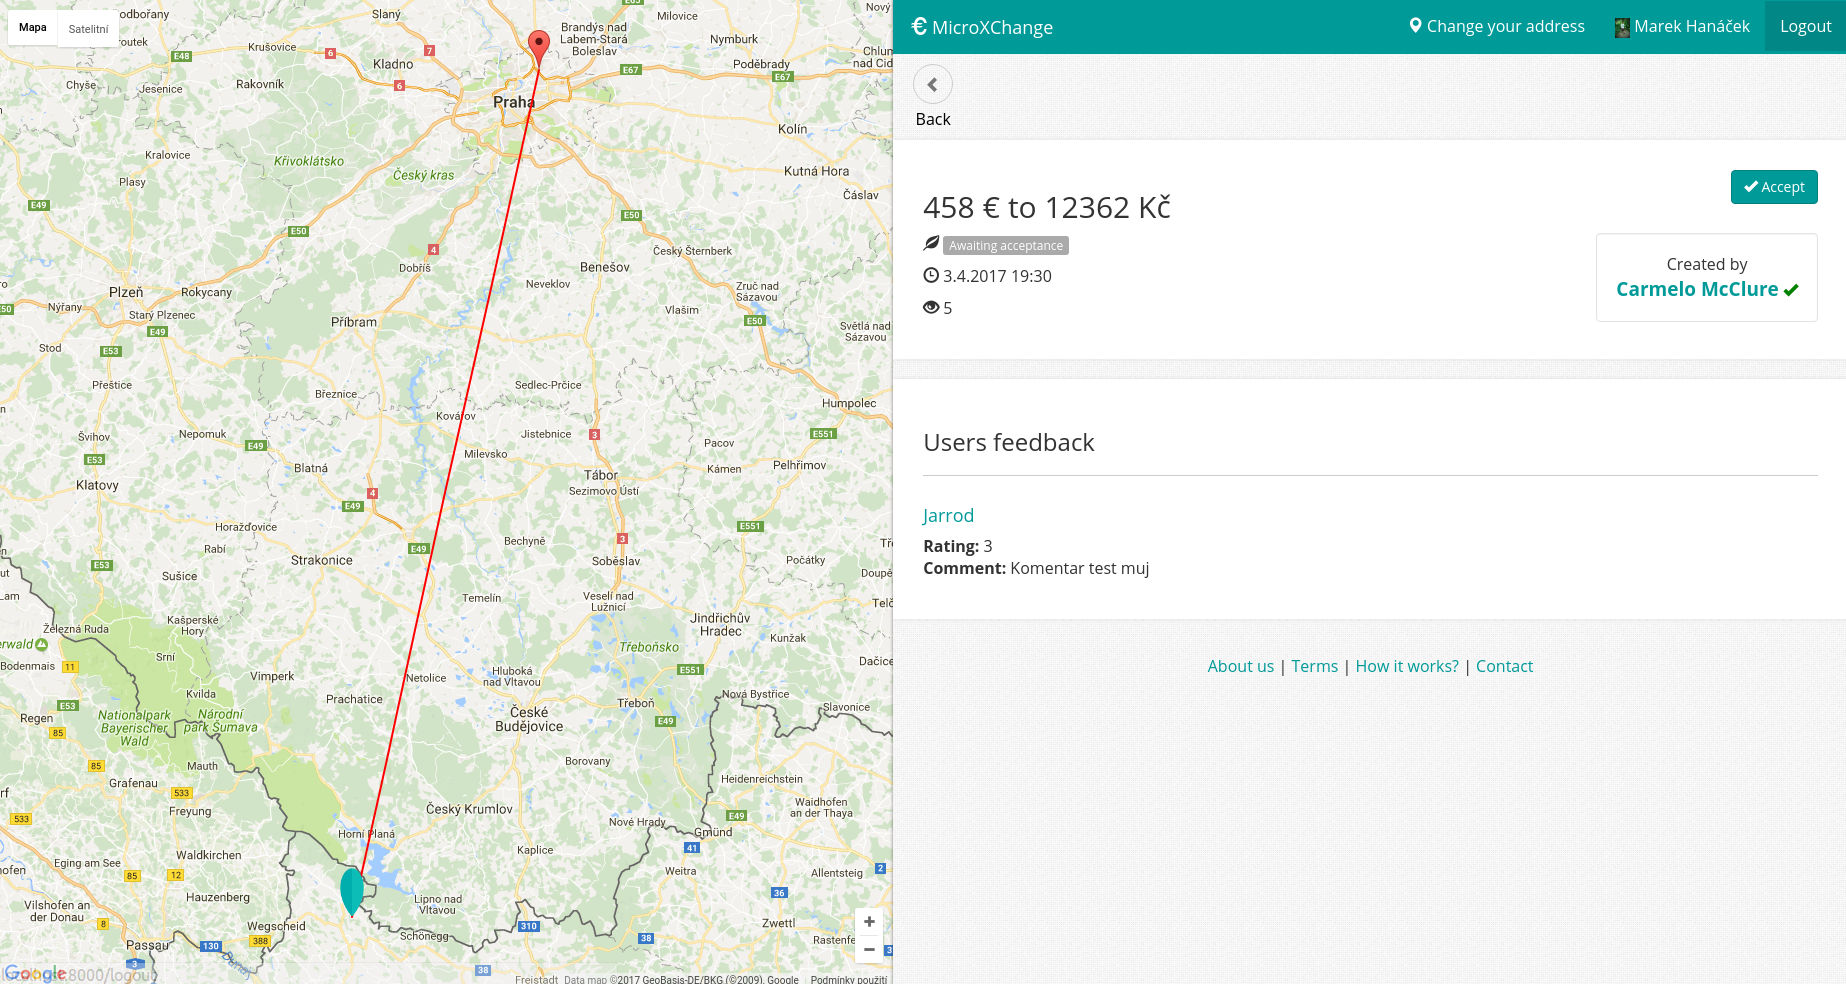
\includegraphics[width=1.0\textwidth]{media/tur/offer-detail-map.png}
    \caption{Detail nabídky s mapou}
    \label{fig:tur:offer-detail-map}
\end{figure}

\subsection{Zobrazení na samostatné stránce}
Toto zobrazení obsahuje totožné informace jako zobrazení s mapou. Při rozvržení bez mapy však máme více prostoru a detail nabídky je tedy uspořádán jinak. Na toto zobrazení se uživatel dostane ze svého uživatelského profilu. Detail nabídky s tímto rozvržením lze vidět na obrázku \ref{fig:tur:offer-detail-no-map}

\begin{figure}[h]
    \centering
    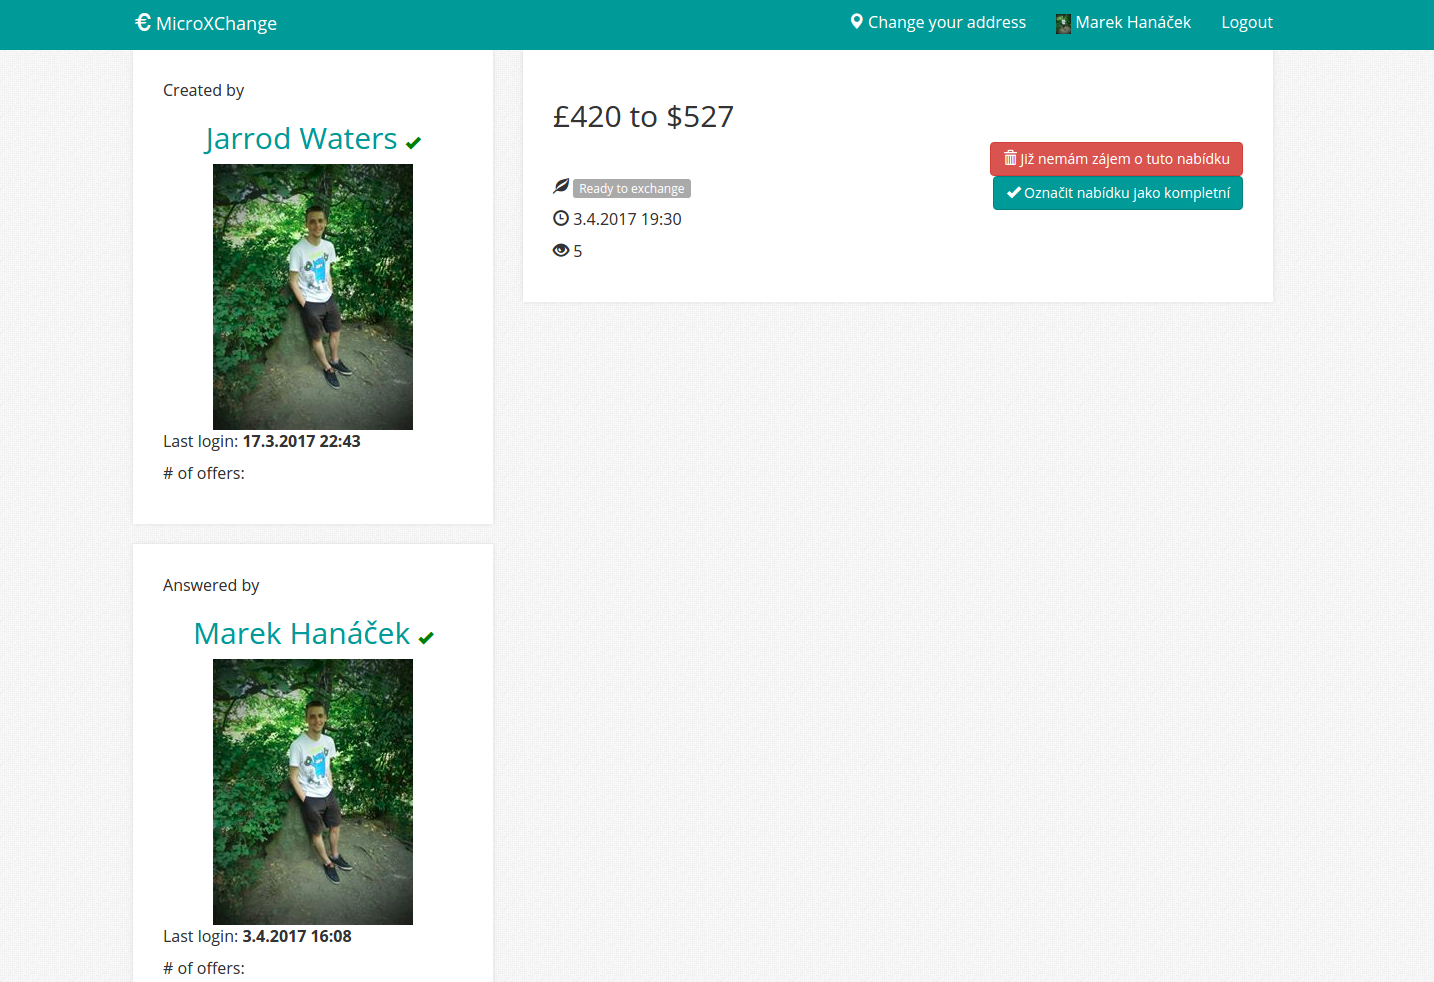
\includegraphics[width=1.0\textwidth]{media/tur/offer-detail-no-map.png}
    \caption{Detail nabídky bez mapy}
    \label{fig:tur:offer-detail-no-map}
\end{figure}